%!TEX root = thesis.tex
\chapter{Infinite Projected Entangled Simplex State}
\label{chapter:ipess}
Introduce to PESS ansatz.

\section{Simplex-solid State}
\label{solidstate}
The simplex-solid state of an SU(N) quantum anti-ferromagnet was derived by Arovas \cite{} and the most significant conclusion is that any simplex states could be described by a natural generalization of the AKLT \cite{} valence bond solid state which means that the bond signlets of the AKLT could be extended to N-site simplices.

The concept of simplex-solid states ansatz were introduce by Xie et al \cite{}. The tensor-network representation of simplex states is called projected entangled simplex state (PESS) which is also considered as an extension of PEPS \cite{} obeying the area law of entanglement entropy and characterizing any states if the dimension of the virtual bonds are large enough. The difference from the PEPS is that the entanglement among the virtual particles is described by entangled simplex tensors which depend on the structure of PESS. For example, in Fig. \ref{fig411}(b) there are three virtual particles within the simplex state, so the entangled simplex tensor $S_{mnl}$ is a rank-3 tensor.

\begin{figure}[ht]
	\centering
	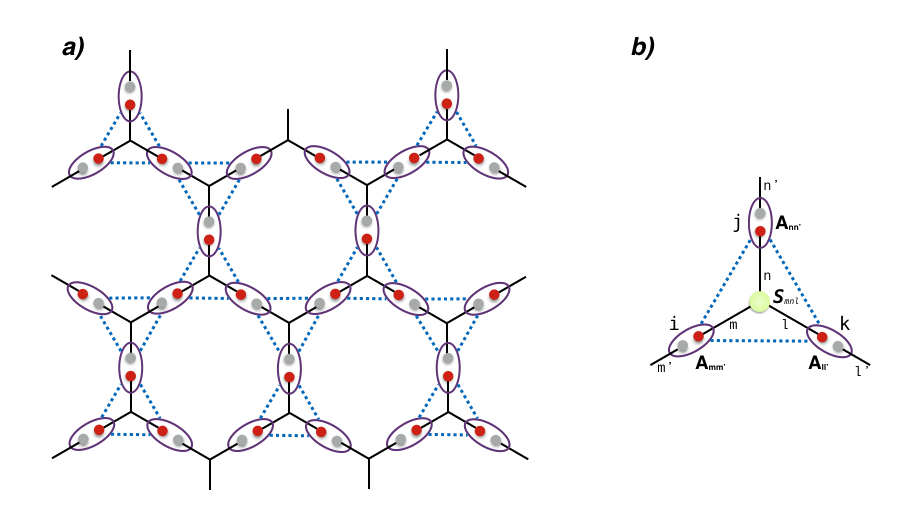
\includegraphics[width=0.80\textwidth]{figures/fig411.png}
	\caption[The picture of the main idea of itebd.]{The red and blue tensor denotes on \textit{odd} and \textit{even} sites. The yellow one are time evolution operators $e^{-\tau H_{k,k+1}}$, $e^{-\tau H_{k+1,k}}$}
	\label{fig411}
\end{figure}

\section{Infinite Kagome Lattice}
In this section, we will discuss about the formulation of the wave function of PESS and employ it as a variational ansatz. In the reference \cite{}, it has shown an example of the spin-2 simplex state on Kagome lattice for illustration. See Fig. \ref{fig411}(a) each physical $S=2$ states on the lattices could be treated as a symmetric superposition of two virtual $S=1$ spins. According to the theory of AKLT, each neighbor simplices (triangles) share a single site symmetrically which also means that the $S=1$ spins could be assigned to one of the simplices (vertex-sharing). Hence, there are three $S=1$ spins in each simplex states. From the features of the $SU(2)$ group, the decomposition of the direct-product of three integer spins is written as, 
\begin{align}
	\label{su2}
	n \otimes n \otimes n = [a_0 \times 0] \oplus \dots \oplus [a_k \times k] \oplus \dots \oplus [a_{3n} \times 3n] \\
	a_k = \begin{cases}
		2k + 1 & \text{, $k \leq n$} \\
		3n + 1 - k & \text{, $k > n$} 
	\end{cases}
	\quad \text{, } k = 0, 1, \dots , 3n ,
\end{align}
where $a_k$ is a constant and $k$ express the $k$th irreducible representation. Now that we can write down the product of the spins in the simplex as,  
\begin{align}
	\label{111}
	\barbelow{1} \otimes \barbelow{1} \otimes \barbelow{1} = \barbelow{0} \oplus \left( 3 \times \barbelow{1} \right) \oplus \left( 2 \times \barbelow{2} \right) \oplus \barbelow{3},
\end{align}
and show that there is an unique spin-singlet state. The result encourage us to define a virtual singlet on simplex,
\begin{align}
	\Ket{\psi_{\alpha}} = \frac{1}{\sqrt{6}} \sum_{\left\{ s_i s_j s_k\right\}}{S^{\alpha}_{s_i s_j s_k}\Ket{s_i, s_j, s_k}},
\end{align}
where $s_i,s_j,s_k$ are $S=1$ virtual spins located at site $i,j$ and $k$ containing in the simplex $\alpha$ and $S^{\alpha}_{s_i s_j s_k}$ is the Levi-Civita antisymmetric tensor $\varepsilon_{ijk}$ [Fig. \ref{fig411}(b)]. For mapping the two virtual $S=1$ spins to the spin-2 subspace, we defined the projection operator $P$ on each site,
\begin{align}
	P = \sum_{s_i,s^{\prime}_{i}}\sum_{s_i,s^{\prime}_{i}}
\end{align}


\subsection{3-PESS}
The example on Kagome lattice.
\label{3pess}

\subsection{5-PESS}
\label{5pess}

\section{Infinite Square Lattice}
The example on Kagome lattice.
\subsection{4-PESS (Rank-3 local tensors)}
\label{4pess2b}

\subsection{4-PESS (Rank-5 local tensors)}
\label{4pess4b}

